\documentclass[12pt, a4paper, oneside]{report}
\usepackage[ngerman]{babel}
\usepackage{graphicx}
\usepackage{mathtools}
\usepackage[citecolor=black, colorlinks=true, urlcolor=blue, linkcolor=black]{hyperref}
    \title{\textbf{Biosphären Mess- und Überwachungsgeräte -- Funktionsprinzipien und Bedienungsanleitung}}
    \author{Tjark Gaudich}
    \date{November 2021}
    
    \addtolength{\topmargin}{-2cm}
    \addtolength{\textheight}{2cm}
\begin{document}
\maketitle

\section{Vorwort}
Das folgende Dokument soll gleichzeitig als Dokumentation und Bedienungsanleitung für die Biosphären Umweltmessgeräte ("die Geräte") dienen, die ich für den Astrobiologie Projektkurs 2021/2022 bei Herr Krobbach entwickelt habe. Damit soll eine Nutzung und Wartung dieser Geräte weit über den Zeitraum meiner Schullaufbahn hinaus ermöglicht werden. Besonderer Fokus wird deshalb auf die Kommunikation mit dem PC zum auslesen der Messwerte gelegt, da dieser vulnerabel für Änderungen des Betriebssystems ist, doch auch alle anderen Aspekte der Geräte sollen so sehr vertieft werden, dass sie ohne großes Vorwissen verstanden und repariert werden können. Sämtliche Quelldateien sind zusammen mit dieser Dokumentation auf 
GitHub\cite{Github} frei zugänglich.
\tableofcontents
\listoffigures

\chapter{Mechanik}

Mechanisch lassen sich die Geräte in vier Komponenten unterteilen:
eine Grundplatte (in \autoref{fig:Querschnitt} Dunkelgrau), an der alle andere Teile und das Glas der Biosphäre befestigt werden, eine Platine mit Sensoren im inneren (nicht gezeigt) und die Hauptplatine (grün) außen sowie ein Deckel (hellgrau), der die Elektronik vor Beschädigungen schützt.
\begin{figure}[h]
	\centering
	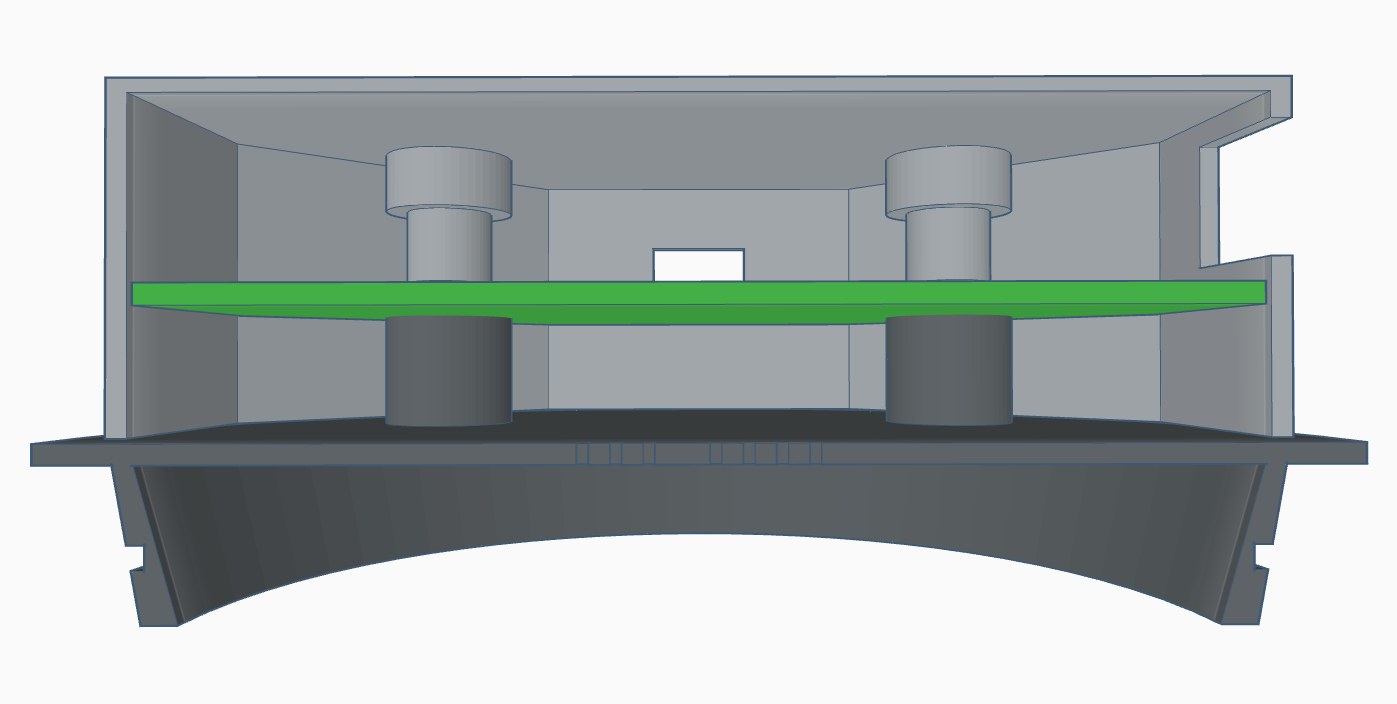
\includegraphics[width=1\textwidth]{Querschnitt}
	\caption{Querschnitt durch das Gerät}
	\label{fig:Querschnitt}
\end{figure}
\\Auf die Platinen wird in \autoref{ch:elektrisch} näher eingegangen, hier reicht es uns zu wissen das die unterer Platine nur über ihren Stecker befestigt wird und die obere ein Achteck von 85mm Durchmesser ist, vier Löcher mit je 50mm Abstand zueinander und 4mm Durchmesser zur Befestigung hat und 1,6mm Dick ist.
\section{Grundplatte}
Entsprechend dieser Maße ist die Oberseite der Grundplatte mit vier Röhren ausgestattet, in die M4 Einschraubmuffen montiert werden. Interessant ist jedoch die Unterseite, die in das Gurkenglas eingeklebt wird. Da die Luftmenge in der Biosphäre konstant ist kommt es bei Temperaturänderungen zu einer Druckänderung nach  dem Gesetz von Amontons \cite[S.~119]{Tafelwerk}, denen die Grundplatte und ihre Verklebung standhalten müssen. $p_0$ und $T_0$ sind dabei Druck und absolute Temperatur beim Verschließen der Biosphäre.
\begin{align}
\frac{p_0}{T_0} = \frac{p_1}{T_1} \footnote{}
\iff \Delta p = T  \times \frac{p_0}{T_0} - p_0
\label{eq:pressure}
\end{align}
Nehmen wir an, das die Biosphäre bei 20°C (293K) und Normaldruck verschlossen wurde und sich im Schlimmsten Falle auf 100°C (373K) aufgeheizt hat (darüber ist ihr Inhalt vermutlich tot, weshalb die Abdichtung irrelevant wird),
\begin{align}
\Delta p = 373K  \times \frac{1013hPa}{293K} - 1013hPa \approx 277hPa
\label{eq:pressure100C}
\end{align}
so ergibt sich nach \autoref{eq:pressure100C} ein Druckunterschied von 277hPa. Diese Druckfestigkeit mit einer Silikon Verklebung zu erreichen ist relativ einfach, beim Übergang zwischen Grundplatte und anschließendem Ring in PLA 3d-Druck Technik wird sie jedoch zu Herausforderung. Um eine höhere Festigkeit zu erreichen wurde dieser Übergang nach dem Druck zusätzlich mit einem Lötkolben verschmolzen. Diese Kombination hielt beim Anschließen eines Kompressors an einen Modifizierten Deckel etwa 300hPa Überdruck stand.

\chapter{elektrisch}
\label{ch:elektrisch}
\chapter{Software}

\begin{thebibliography}{9}

\bibitem{Github}
  Tjark Gaudich,
  \textit{\url{https://github.com/TjarkG/biosphere-monitor}},
  GitHub.com,
  2021
  
\bibitem{Tafelwerk}
  Prof. Dr. Lothar Meyer et al.,
  \textit{Das große Tafelwerk interaktiv 2.0},
  Cornelsen Verlag, Berlin,
  1.Auflage, 8. Druck 2018

\end{thebibliography}

\end{document}